\documentclass[x11names]{article}
\usepackage[a4paper, total={6in, 9in}]{geometry}
\usepackage[skins]{tcolorbox}
\usepackage{tikz}
\usetikzlibrary{arrows}
\usetikzlibrary{calc}
\usepackage{pgfplots}
\pgfplotsset{compat=1.9}
\usepgflibrary{shapes.geometric}
\usepackage{xcolor}
\usepackage{amsmath}
%\usepackage{fouriernc}
\usepackage{mathrsfs}
\usepackage{amssymb}
\usepackage{hyperref}
\usepackage{enumitem}

%% custom
\renewcommand*\contentsname{Indice}
\setcounter{tocdepth}{4}
\setcounter{secnumdepth}{2}
\pgfplotsset{compat=1.15}

% boxes
\definecolor{myblue}{RGB}{224, 245, 255} 
\definecolor{myred}{RGB}{198, 247, 211} 
\definecolor{myorange}{RGB}{255, 102, 0} 

\newtcolorbox{es}[2][]{%
	enhanced,sharp corners,boxrule=0.4pt,colback=white, colframe=black, coltitle=black,fonttitle=\itshape, 
	attach boxed title to top left={yshift=-0.5\baselineskip-0.4pt,xshift=2mm},
	boxed title style={tile, size=minimal, left=0.5mm, right=0.5mm,
		colback=white, before upper=\strut, boxrule=0.5pt, colframe=black},
	title=#2,top=1em,#1 
}
\newtcolorbox{dym}[2][]{%
	enhanced,colback=white,colframe=black,coltitle=black,
	sharp corners,boxrule=0pt, %0.4pt
	fonttitle=\itshape,,
	attach boxed title to top left={yshift=-0.5\baselineskip-0.4pt,xshift=2mm},
	boxed title style={tile,size=minimal,left=2.5mm,right=0.5mm,
		colback=white,before upper=\strut},
	title=#2,top=1em,#1
}
\newtcolorbox{blues}[2][]{%
	enhanced,colback=myblue,colframe=black,coltitle=black,
	sharp corners,boxrule=0.4pt,
	fonttitle=\bfseries\itshape,
	attach boxed title to top left={yshift=-0.5\baselineskip-0.4pt,xshift=2mm},
	boxed title style={tile,size=minimal,left=0.5mm,right=0.5mm,
		colback=myblue,before upper=\strut},
	title=#2,top=1em,#1
}
\newtcolorbox{redes}[2][]{%
	enhanced,colback=myred,colframe=black,coltitle=black,
	sharp corners,boxrule=0.4pt,
	fonttitle=\bfseries\itshape,
	attach boxed title to top left={yshift=-0.5\baselineskip-0.4pt,xshift=2mm},
	boxed title style={tile,size=minimal,left=0.5mm,right=0.5mm,
		colback=myred,before upper=\strut},
	title=#2,top=1em,#1
}
\newtcolorbox{coroll}[2][]{%
	enhanced, colback=white, colframe=black, coltitle=black,
	sharp corners, boxrule=0pt,
	fonttitle=\bfseries\itshape,
	attach boxed title to top left={yshift=-0.5\baselineskip-0.4pt,xshift=2mm},
	boxed title style={tile,size=minimal,
		left=1mm, right=1mm, % Horizontal padding
		top=1mm, bottom=1mm, % Vertical padding
		colback=myred,
		before upper=\strut},
	title=#2,top=1em,#1
}

\newcommand*{\QEDA}{\null\nobreak\hfill\ensuremath{\blacksquare}}%
\newcommand*{\QEDB}{\null\nobreak\hfill\ensuremath{\square}}%

\newcommand{\esempio}[2]{
	\begin{es}{esempio #1}
		#2
	\end{es}
}
\newcommand{\definizione}[2]{
	\begin{center}
		\fboxsep11pt
		\colorbox{myblue}{\begin{minipage}{5.75in}
				\begin{blues}{Definizione: #1}
					#2
				\end{blues}
		\end{minipage}}
	\end{center}
}
\newcommand{\teorema}[2]{
	\begin{center}
		\fboxsep11pt
		\colorbox{myred}{\begin{minipage}{5.75in}
				\begin{redes}{#1}
					#2
				\end{redes}
		\end{minipage}}
	\end{center}
}
\newcommand{\dimostrazione}[2]{
	\begin{dym}{\(\cdots\)dimostrazione#1 \(\cdots \cdots \cdots \cdots \cdots \cdots \cdots \cdots \cdots\cdot\cdots\cdots\cdots\cdots\cdots\cdots\cdots\cdots\cdots\cdots\cdots\cdots\cdots\cdots\cdots\cdots\)}
		#2
		\QEDB
	\end{dym}
}
\newcommand{\corollario}[2]{
	\begin{center}
		\begin{coroll}{corollario#1}
			#2
		\end{coroll}
	\end{center}
}

\pgfplotsset{my axis/.append style={height=9cm,width=9cm,grid=major,samples=100,yticklabel=\empty,xticklabel=\empty}}
\pgfplotsset{my plot/.append style={thick,samples=500}}

\begin{document}
	
\begin{titlepage}
	\begin{center}
		\vspace*{1cm}
		
		\textbf{\LARGE Relazione di laboratorio - Pendolo semplice}
		
		\vspace{0.3cm}
		\large \textit{Misura del periodo di un pendolo semplice} \\
		
		\vspace{0.5cm}
		\Large Federico Cesari \\
		
		\small 1096759 
		\vspace{0.2cm}
		
		\small Gruppo 5
		
		
		\vspace{3cm}
		\begin{center}
			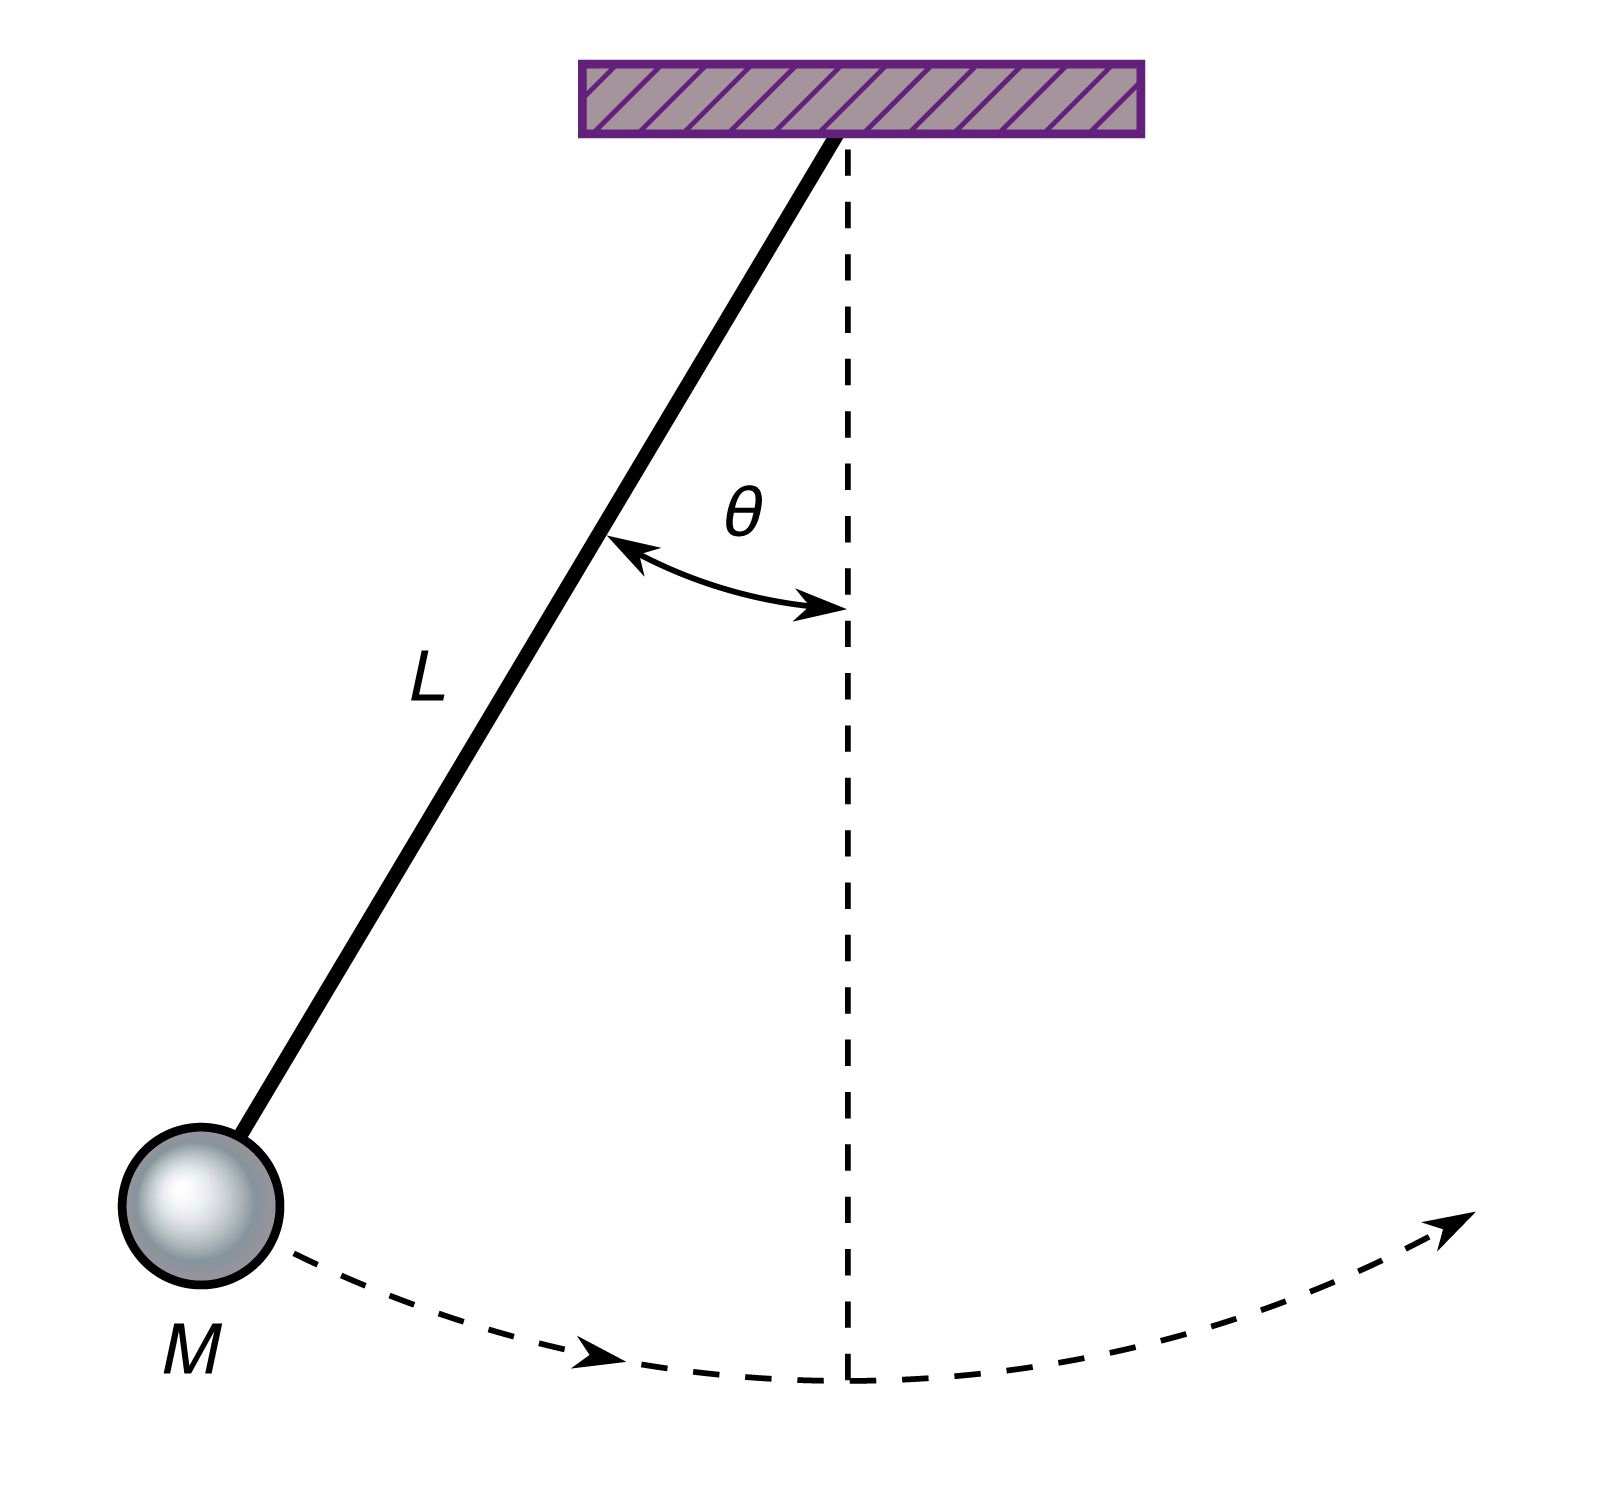
\includegraphics[scale=0.1]{IMG_0200.jpeg}	
		\end{center}
		
		
		
		\vfill
		
		
		
		corso A\\
		Università degli studi di Torino, Torino\\
		4 aprile 2024\\
		
		
	\end{center}
\end{titlepage}
\tableofcontents
\newpage
	
	
\section{Successioni di funzioni}

%\begin{center}
%\begin{tikzpicture}
%	\begin{axis}[my axis,xmin=-1,xmax=1]
%		\addplot[my plot, domain y=-pi/2:pi/2] {atan(x)};
%		\addplot[my plot, domain y=-pi/2:pi/2] {atan(2*x)};
%		\addplot[my plot, domain y=-pi/2:pi/2] {atan(20*x)};
%	\end{axis}
%\end{tikzpicture}
%\end{center}

\[ 
A \subseteq \mathbb{R} \;\ (\text{o } \mathbb{C}), \;\ f_{n}: A \to \mathbb{R} \;\ (\text{o } \mathbb{C}), \;\ n \in \mathbb{N} 
\]
\[ 
\begin{array}{ccl}
	N & \to & \{\text{f.ni definite su } A\} \\
	n & \mapsto & f_{n}
\end{array}
\]
Vogliamo studiare come si comporta \((f_{n})_{n}\) quando \(n\to +\infty\).

\subsection{Limiti di successioni}


\definizione{Convergenza puntuale}
{Diciamo che la successione di funzioni \((f_{n})_{n}\), \(f_{n}:A\subseteq \mathbb{R}\to \mathbb{R}  (\text{o } \mathbb{C})\) \textbf{converge puntualmente} (o semplicemente) a una funzione  \(f\) sull'insieme \(E \subseteq A\) se 
\[ 
\forall x \in E, \;\ \lim_{n\to + \infty}f_{n}(x) = f(x)
\]
Notiamo che quest'ultimo limite è un limite di successione numerica, quindi
\[ 
\forall x \in E, \quad  \forall \varepsilon > 0 \;\ \exists \bar{n} = \bar{n}(\varepsilon,x) \;\ \text{t.c.} \;\ |f_{n}(x) - f(x)| < \varepsilon, \quad \forall n \geq \bar{n}
\]}

\definizione{Convergenza uniforme}{Diciamo che la successione di funzioni \((f_{n})_{n}\), \(f_{n}:A\to \mathbb{R}  \;\ (\text{o } \mathbb{C})\) \textbf{converge uniformemente} su \(E \subseteq A\) alla funzione \(f:E\to \mathbb{R}\) se
\[ 
\forall \varepsilon > 0 \quad \exists \bar{n} = \bar{n}(\varepsilon) \;\ \text{t.c.} \;\ |f_{n}(x) - f(x)| < \varepsilon \quad \forall n \geq \bar{n}
\]
equivalentemente
\[ 
\forall \varepsilon > 0 \quad \exists \bar{n} = \bar{n}(\varepsilon) \;\ \text{t.c.} \;\ \text{sup}|f_{n}(x) - f(x)| < \varepsilon \quad \forall n \geq \bar{n}
\]
dove l'estremo superiore viene denominato \(\alpha_n\) successione positiva (\(\geq 0\)):
\[ 
\forall \varepsilon > 0 \quad \exists \bar{n} = \bar{n}(\varepsilon) \;\ \text{t.c.} \;\ 0 \leq \alpha_n < \varepsilon \quad \forall n \geq \bar{n}
\]
opure
\[ 
\
\]
} 


\esempio{1}{}
\esempio{2}{}
\esempio{3}{}



\teorema{Teorema 1 - La convergenza unifore preserva la continuità}{
Sia \((f_{n})_{n}\) una successione di funzioni \(f_{n}:A\subseteq \mathbb{R}\to \mathbb{R} \;\ (\text{o } \mathbb{C})\) tali che
\begin{enumerate}[start=1,label={(\itshape H\arabic*)}]
	\item \(f_{n}\) sono funzioni continue su \(E\subseteq A\),
	\item \(f_{n}\) converge uniformemente a \(f\) su \(E\)
\end{enumerate}
allora \(f\) è continua su \(E\)
}
\dimostrazione{}{
La tesi è 
\[ 
\forall x_{0} \in E, \;\ \lim_{x\to x_{0}} f(x) = f(x_{0})
\]
ovvero che
\[ 
\forall x_{0} \in E \qquad \forall \varepsilon > 0 \;\ \exists \delta = \delta(x_{0},\varepsilon) \;\ \text{t.c.} \;\ |f(x) - f(x_{0})| < \varepsilon \qquad \forall x \in (x_{0}-\delta,x_{0}+\delta) \cap E 
\]
\begin{itemize}
	\item Da (\textit{H2}) convergenza uniforme sappiamo che \( \lim_{n\to + \infty} \alpha _{n} = 0\) quindi 
	\[\exists \hat{n} = \hat{n}(\varepsilon) \;\ : \;\ \alpha_{n} = \text{sup}|(f_{n}(x) - f(x))| < \frac{\varepsilon}{3} \quad \forall n\geq\hat{n}
	\]
	\item Da (\textit{H1}) abbiamo invece la continuità di \(f_{\hat{n}}\) in \(x_{0}\):
	\[ 
	\exists \delta = \delta(x_{0},\varepsilon) \;\ : \;\ | f_{\hat{n}}(x) - f_{\hat{n}}(x_{0}) | < \frac{\varepsilon}{3} \;\ \forall x \in I_{\delta}
 	\]
 	Ora utilizzando la riscrittura
 	\begin{align*}
 		| f(x) - f(x_{0}) |  =& | f(x) - f_{\hat{n}}(x) + f_{\hat{n}}(x)  - f_{\hat{n}}(x_{0}) + f_{\hat{n}}(x_{0}) - f(x_{0})| \\
 		\leq & |f(x) - f_{\hat{n}}(x)| + |f_{\hat{n}}(x) -f_{\hat{n}}(x_{0})| + |f_{\hat{n}}(x_{0}) - f(x_{0})| \\
 		= & \frac{\varepsilon}{3} + \frac{\varepsilon}{3} + \frac{\varepsilon}{3}  = \varepsilon
 	\end{align*}
\end{itemize} }

\teorema{Teorema 2 - Passa al limite sotto integrale}{
Sia \((f_{n})_{n}\) una successione di funzioni \(f_{n}:[a,b]\to \mathbb{R}\) tale che
\begin{enumerate}[start=1,label={(\itshape H\arabic*)}]
	\item \(f_{n}\) sono funzioni continue su \([a,b]\),
	\item \(f_{n}\) converge uniformemente su \([a,b]\)
\end{enumerate}
allora 
\[ 
\lim_{n\to+\infty} \int_{a}^{b}f_{n}(x) \: dx \quad = \quad \int_{a}^{b}\lim_{n\to+\infty} f_{n}(x) \quad = \quad \int_{a}^{b}f(x) \: dx
\]
}
\dimostrazione{}{
Dal \textit{\textbf{Teorema 1}} sappiamo che \(f\) è continua su \([a,b]\) e perciò è integrabile è 
\[ 
\int_{a}^{b}f(x)\: dx
\]
è ben definito.

Vogliamo dimostrare che
\[ 
\lim_{n\to+\infty}\int_{a}^{b}f_{n}(x)\: dx = \int_{a}^{b}f(x)\: dx 
\]
ovvero che 
\[ 
\forall \varepsilon > 0 \;\ \exists\tilde{n} = \tilde{n}(\varepsilon) \;\ : \;\ |I_{n} - I| < \varepsilon \;\ \forall n \geq \tilde{n}
\]
Utilizziamo la disugualianza
\begin{align*}
	|I_{n} - I|  = \left|\int_{a}^{b}f_{n} - \int_{a}^{b}f\right| =& \left|\int_{a}^{b}f_{n} - f\right| \\
    \leq & \int_{a}^{b}|f_{n} - f | \\
	\leq & \int_{a}^{b} \alpha_{n} = \alpha_{n}(b-a)
\end{align*}
e poiché per \textit{(H2)} si ha \(\alpha_{n} \to 0\) 
\[ 
\exists\tilde{n} : \alpha_{n}(b-a) < \varepsilon \;\ \forall n \geq \tilde{n}
\]
}

\esempio{4}{}

\teorema{Teorema}{
Sia \((f_{n})_{n}\), \(f_{n}:A\subseteq \mathbb{R}\to \mathbb{R}\) (o \(\mathbb{C}\)) tale che 
\begin{itemize}
	\item \(f_{n}\) converga uniformemente a \(f\) in \(E \subseteq A\),
	\item \(f_{n}\) siano continue sulla chiusura di \(E\): \(\bar{E}\)
\end{itemize}
allora si ha che \(f_{n}\) converge uniformemente a \(f\) su \(\bar{E}\).
}


% SERIE DI FUNZIONI
\newpage
\section{Serie di funzioni}
Presa \((f_{n})_{n}\) successione di funzioni, \(f_{n}:A\subseteq \mathbb{R} \to \mathbb{R}\) (o \(\mathbb{C}\)), chiamiamo 
\[ 
\sum_n f_{n}(x)
\]
\textbf{serie di funzioni}. Definiamo
\[ 
S_{N} = \sum_{n=1}^N f_{n}(x)
\]
successione delle ridotte.
\paragraph*{Convergenza della serie} Diciamo che la serie converge (puntualmente o uniformemente) su un insieme \(E\subseteq A\) se lo fa la successione delle ridotte. Si andrà quindi a studiare il limite di \(S_{N}\) che chiamiamo somma della serie.

\teorema{Teorema 1S}{
Data \(f:A\subseteq \mathbb{R} \to \mathbb{R}\), se
\begin{itemize}
	\item \(f_{n}\) continue su \(E\subseteq A\);
	\item \(\sum_n f_{n}\) converge uniformemente su \(E\subseteq A\) alla somma \(S(x)\)
\end{itemize}
Allora \(S(x)\) è continua su \(E\).}
\teorema{Teorema 2S}{
Data \(f:A\subseteq \mathbb{R} \to \mathbb{R}\) e \(E = [a,b]\subseteq \mathbb{R}\), se
\begin{itemize}
\item \(f_{n}\) continue su \(E\subseteq A\);
\item \(\sum_n f_{n}\) converge uniformemente su \(E\subseteq A\) alla somma \(S(x)\)
\end{itemize}
Allora
\[ 
\int_{a}^{b} \sum f_{n}(x)dx \quad  = \quad \sum \int_{a}^{b}  f_{n}(x)dx 
\]}

\definizione{}{
	\[ 
	I_{s} = \left\{x \;\:\;\ \text{la serie considerata} \sum f_{n}(x) \text{converge semplicemente} \right\}
	\]
	per la serie \(\sum x^n\) si ha che \(I_{s} = (-1,1)\)
	\[ 
	I_{a} = \left\{x \;\:\;\ \text{la serie considerata} \sum |f_{n}(x)| \text{converge semplicemente} \right\}
	\]
}

\teorema{Teorema: m-test o criterio di convergenza totale}{
Date 
\begin{itemize}
	\item \((f_{n})_{n}\) successione di funzioni su \(E\subseteq \mathbb{R}\) (o in \(\mathbb{C}\));
	\item \((m_{n})_{n} \subseteq \mathbb{R}\) successione di numeri reali positivi. 
\end{itemize}
tali che
\begin{enumerate}[start=1,label={(\itshape H\arabic*)}]
	\item \(|f_{n}(x)|\leq m_{n}\) \(\forall x \in E\), \(\forall n\);
	\item \(\sum m_{n}(x) < + \infty\).
\end{enumerate}
Allora la serie \(\sum f_{n}(x)\) converge assolutamente in ongi punto di \(E\) è uniformemente su \(E\) \(\implies\) la serie converge totalmente.}


\teorema{Teorema 3S}{
	Data \(f:A\subseteq \mathbb{R} \to \mathbb{R}\) (o \(\mathbb{C}\)). Se
	\begin{itemize}
		\item \(\sum_n f_{n}\) converge uniformemente su \(E\),
		\item \(f_{n}\) sono continue su \(\bar{E}\)
	\end{itemize}
	allora \(\sum_n f_{n}\) converge uniformemente su \(\bar{E}\).
}

\subsection{Serie di potenze in \(\mathbb{C}\)}
Intendiamo con serie di potenze in \(\mathbb{C}\) un espressione del tipo
\[ 
\sum_{n\geq 0}a_{n}(z-z_{0})^n
\]
dove \((a_{n})_{n}\) è una successione di numeri complessi, \(z_{0} \in \mathbb{C}\) è il \textit{centro} e \(z\) è la variabile complessa. I concetti di convergenza si estendono sostituendo il modulo al valore assoluto nelle relative definizioni.

In campo complesso l'intervallo di convergenza viene sostituito da un \textbf{disco di convergenza}. \\

\noindent
La successione delle ridotte \(S_{N}(z)\) è un polinomio di grado \(N\) a variabile complessa.

\teorema{Teorema: disco di convergenza}{
Data una serie di potenze in \(\mathbb{C}\), \(\sum_{n\geq 0} a_{n}(z- z_{0})^n\), esiste \(R\geq 0\) detto raggio dei convergenze della serie tale che
\begin{enumerate}
	\item La serie \textbf{converge assolutamente} in \(D_{R}(z_{0}) = \{z\in \mathbb{C} : |z-z_{0}| < R\}\),
	\item la serie \textbf{non converge semplicemente} in \(\mathbb{C} \setminus \overline{D_{R}(z_{0})}\),
	
	\[ 
	D_{R}(z_{0}) \subseteq I_{a} \subseteq I_{s} \subseteq \overline{D_{R}(z_{0})}
	\]
	
	\item la serie \textbf{converge uniformemente} su ogni \(\overline{D_{r}(z_{0})}\) con \(r \in (0,R)\).
\end{enumerate}
}
\dimostrazione{}{
Per prima cosa sappiamo che \(z_{0} \in I_{s}\) quindi \(I_{s} \neq \varnothing\).

Definiamo 
\[ 
R := \text{sup}\{|z-z_{0}| : z \in I_{s}\}
\]
Ora andiamo a studiare quando \(R\) si annulla e quando è maggiore di zero:
\begin{itemize}
	\item \(\boxed{R = 0} \quad\) Se \(R\) è nullo il punto \(z_{0}\) corrisoponde all'insieme \(I_{s}\): 
	\[ 
	\{z_{0}\} = I_{s}
	\]
	La serie converge solo in un punto dove si riduce al primo termine \(a_{0}\), quindi \(I_{a} = I_{s}\).
	\item \(\boxed{R > 0} \quad\) e \(r \in (0,R)\).
	
	Avendo definito \(R\) come il \textit{raggio dell'insieme} \(I_{s}\) di centro \(z_{0}\), il punto \(2\) è subito dimostrato.
	
	\begin{itemize}
		\item considero \(\boxed{z_{1}:|z_{1} - z_{0}| \in (r,R)}\). Si ha che \(z_{1} \in I_{s}\) ovvero
		\[ 
		\sum_{n\geq 0} a_{n}(z_{1}-z_{0})^n \quad \text{convergente in } \mathbb{C}
		\]
		\begin{align*}
			\implies& \lim_{n\to +\infty}a_{n}(z_{1}-z_{0})^n = 0 \\ 
			\implies& \exists\tilde{n} \;\ : \;\ |a_{n}(z_{1}-z_{0})^n| < 1 \;\ \forall n \geq \tilde{n}
		\end{align*}
		
		\item considero \(\boxed{z \in \overline{D_{r}(z_{0})}} \quad\). Vogliamo usare l'm-test per dedurre la convergenza assoluta in ongi \(\overline{D_{r}(z_{0})}\) e la convergeza uniforme in \(D_{r}(z_{0})\).
		
		Vogliamo maggiorare
		\[ 
		|a_{n}(z_{1}-z_{0})^n|
		\]
		con un numero \(m_{n}\) tale che \(\sum m_{n} < +\infty \;\ \forall t \in \overline{D_{r}(z_{0})}\):
		\[ 
		|a_{n}||(z_{1}-z_{0})^n| \leq |a_{n}|r^n\frac{|(z_{1}-z_{0})^n|}{}
		\]
	\end{itemize}
\end{itemize}
}
\corollario{}{
corpo
}
	
\end{document}